\chapter{Úvod}
Vývoj centrálního zásobování teplem prošel od dob svého vzniku několika fázemi.
Z hlediska dnešní doby je nejvýznamnější výměna starých parovodů za
prefabrikované horkovody, čímž dochází ke snížení přestupu tepla z rozvodů do
jejich okolí a snížení nákladů při stavbě nových částí sítě. Z hlediska
několika budoucích dekád je žádoucí transformace na obnovitelné, plně
udržitelné a efektivní zásobování teplem. To přináší nové technologické výzvy
související zejména s integrací obnovitelných zdrojů, využitím odpadního tepla
a celkově snižováním emisí oxidu uhličitého. Je totiž obecně přijímaným faktem,
že pro smysluplnou implementaci obnovitelných zdrojů tepla a odpadní, jež lze
obecně považovat za nízkoteplotní zdroje, je nutné dále snižovat
teplotu v teplárenských rozvodech. Snižovaní této teploty má za následek další
redukci ztrát při distribuci tepla, ale komplikuje efektivní předávání tepla na
straně spotřebitelů a zvyšuje provozní náklady čerpadel. Proto je nutné do sítě
implementovat další prvky, jež umožní efektivní zvýšení teploty blízko
samotných spotřebitelů. Jako další problém lze zmínit značnou nestálost
obnovitelných zdrojů tepla. Se zvyšující se komlexností sítí bude nutné zlepšit
možnosti optimalizace jejich provozu. Toho lze dosáhnout například prediktivním
řízením využívající matematické modely a vhodnou koncepcí akumulace tepla
společně s předpovědí počasí a predikcí množství potřebného tepla. Systémy, jež
se budou schopny vypořádat s těmito a dalšími výzvami lze obecně nazvat čtvrtou
generací teplárenských sítí \cite{Lund2014}.

Množství hmoty, které ovlivňuje fyzikální dynamiku rozsáhlých energetických
systémů již samo o sobě naznačuje komplexnost potenciálního matematického
modelu (digitálního dvojčete či prototypu). Užitečnost takových modelů roste
společně s jejich výpočtovou rychlostí a také s rychlostí s jakou je možné tyto
modely sestavovat. Deklarativní programování může výrazně zjednodušit proces
kompletace z jednotlivých komponent. V numerickém řešení pak modely obvykle
využívají matice, jež se v nich objevují zpravidla kvůli tzv. linearizaci
diferenciálních rovnic (tedy rovnic řídících fyzikální chování). Výpočtová
rychlost je pak úměrná velikosti a hustotě těchto matic. V dnešní době se
můžeme často setkat se snahou o zmenšování matic pomocí redukce směrem k tzv.
jedno‑dimenzionálním modelům. Další výrazný vliv na výpočetní rychlost má
programovací jazyk použitý pro implementaci (strojový kód zpravidla poběží
rychleji než kód interpretovaný) a také míra a provedení paralelizace
algoritmů.

Počítačové učení je moderní vědecká disciplína, která umožňuje vytvářet modely
pomocí dat a to na základě optimalizace parametrizovaných programů. V této
oblasti existuje celá řada numerických struktur umožňující až univerzální
aproximaci (např. neuronové sítě).

Cílem této disertační práce je vytvoření nástrojů (softwarových balíčků) pro
modelování komponent tepelného zásobování s ohledem na optimalizaci numerické
efektivnosti simulací s využitím deklarativního programování a počítačového
učení. Model tepelného zásobování zde poslouží jako studijní příklad jejich
aplikace.

\chapter{Abstrakt}
\label{abstrakt}
Text abstraktu.

\chapter{Současné shrnutí stavu poznání}
\label{struktura}
V této kapitole jsou uvedeny relevantní rovnice pro modelování CZT. Dále je
provedena stručná rešerše literatury na kterou tato práce navazuje, nebo
využívá její poznatky. Následně jsou popsány použitelné výpočetní přístupy
a metody spolu s aspekty, ovlivňující numerickou efektivnost simulací.

\section{Stručná historie rozvoje teplárenství}
\label{sec:history}
Teplárenské potrubí slouží k dopravě tepla od jeho výrobce k jeho spotřebiteli
pomocí teplonosného média. V minulosti se jako první teplonosné médium
používala pára o teplotě i přes 240 °C. Tyto rozvody generovaly značné tepelné
ztráty a kvůli vysokému tlaku (naakumulované tlakové energii) i vážné
explozivní nehody. Kvůli kondenzaci páry ve vratném potrubí docházelo k jeho
korozi. Pára se jako hlavní teplonosné médium stále využívá například v Paříži
či Manhattanu. Nástupce tohoto provedení využíval tlakovou horkou vodu o
teplotě přes 100 °C. Kvůli nestlačitelnosti vody se výrazně omezily explozivní
nehody.
Motivací bylo snížení tepelných ztrát a možnost lepší implementace kombinované
výroby tepla a elektrické energie v městských oblastech. Poté přišel trend
snižování teploty v rozvodech pod 100 °C. Stále byla využívána tlaková horká
voda. Začalo se značně využívat prefabrikované a před-izolované potrubí
snižující množství lidské práce při výstavbě a obnově rozvodů. Začala se
využívat lokální paliva, odpady a na několika místech i sluneční či geotermální
energie.

V následujících dvou až třech dekádách bude trend snižování teploty v
rozvodech pokračovat ruku v ruce se snižující se náročností budov na prostorové
vytápění. Bude existovat snaha o výraznější implementaci obnovitelných a
odpadních zdrojů energie a k využívání synergií. Pro snížení následků fluktuací
zdrojů, budou využívány akumulační systémy a matematické modely jednotlivých
součástí systému se zaměřením na jejich dynamiku jakožto základ prediktivního
řízení využívající předpovědi meteorologických podmínek \cite{Lund2014}.

\section{Tepelná dynamika teplárenských rozvodů/potrubí}
\label{sec:HeatDynamics}
Moderní teplárenské systémy pracují s teplonosným médiem v kapalném skupenství.
Fluidní dynamika je prostorovým fenoménem, ale lze zavádět zjednodušující
předpoklady odpovídající kontextu aplikace. Při uvažování zjednodušené fyziky
proudění tekutiny v potrubí (tj. na nestlačitelné a jedno-dimenzionální
proudění) lze problém zjednodušit na součinnost třech fyzikálních jevů:

\begin{itemize}
  \item Advekce veličin jež jsou unášeny proudem podél potrubí
  \item Difúze veličin v tekutině podél potrubí
  \item Příspěvky do veličin vnitřními a/či externími zdroji
\end{itemize}

\begin{figure}[h] \capstart
  \label{fig:heatwave}
  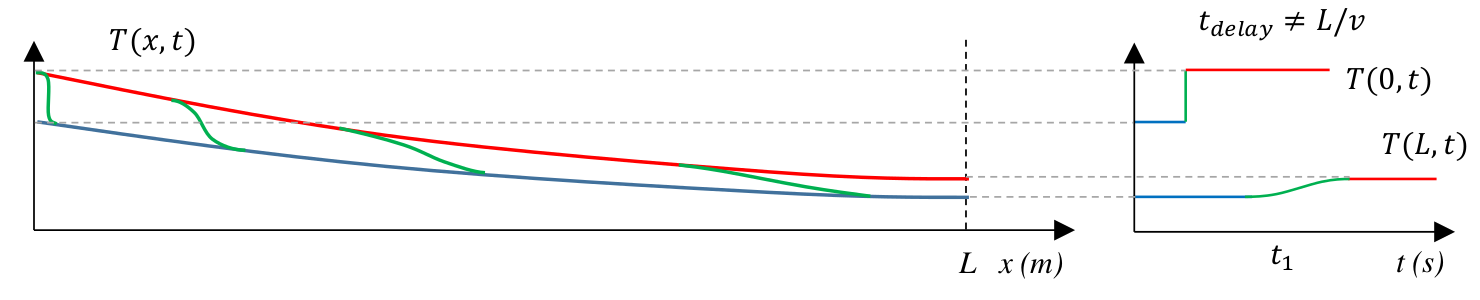
\includegraphics[width=\textwidth]{figures/heat_front}
  \caption{Proces šíření teplotní vlny v potrubí}
\end{figure}

Parciální diferenciální rovnice (PDR) pro celkovou dynamiku je pak v tomto
kontextu následující:
\begin{equation}
  \label{eq:AdvDiff}
  \frac{dy}{dt} = -u \frac{dy}{dx} + D\frac{d^{2}y}{dx^2} + {S_y}
\end{equation}
kde \(y\) je unášená veličina, \(t\) je čas, \(x\) je podélná poloha, \(u\) je
rychlost tekutiny, \(D\) je celkový koeficient difúze a \(S_y\) je celkový
zdroj unášené veličiny. Z hlediska tepelného chování může být touto veličinou
měrná entalpie, ale lze pracovat i s teplotou.

\begin{itemize}
  \item
    \textbf{Advekce} je jev, při kterém se transportují veličiny (jsou unášeny)
    ve směru objemového pohybu. Tento jev ovlivňuje tepelnou dynamiku nejvíce,
    neboť z velké části určuje čas transportu (zpoždění) teplotní fronty.
  \item
    \textbf{Axiální difúze} je složena jednak z difúze kondukcí tepla v
    tekutině a dále z tzv. turbulentního míchání v axiálním směru. Difúze
    způsobená kondukcí je u teplárenských rozvodů zanedbatelná
    \cite{VanderHeijde2017a,VanderHeijde2017b}. Za to turbulentní difúze roste
    přibližně lineárně s Reynoldsovým číslem \cite{Chertkov2018}. Axiální
    difúze způsobuje rozpínání (vyhlazování) teplotní fronty, což znamená,
    že náhlé změny na vstupu do potrubí se projevují pozvolnými změnami na jeho
    konci. V případě uvažování horizontálně uloženého potrubí lze tímto
    způsobem zahrnout i vliv gravitace. Axiální difúze nemá vliv na zpoždění
    teplotní fronty, ale výrazně ovlivňuje její tvar.
  \item
    \textbf{Zdrojový termín} \(S_y\) zahrnuje především výměnu tepla mezi
    tekutinou a vnitřním povrchem přilehlé stěny ve kterém tekutina proudí (což
    v důsledku určuje vliv akumulace tepla na vývoj teplotní fronty). Velikost
    hustoty tepelného toku je závislá na rozdílu teploty vody a povrchu,
    vlastnostech tekutiny, velikosti a drsnosti povrchu a na rychlosti
    proudění. Výměna tepla ovlivňuje jak zpoždění teplotní fronty tak její
    tvar. Tuto intenzitu lze vyjádřit rovnicí pro konvekci tepla
    \ref{eq:ConvHeatTransfer}.
\end{itemize}

\begin{equation}
  \label{eq:ConvHeatTransfer}
  Q = \alpha S \Delta T
\end{equation}
kde \(Q\) je tepelný tok ze stěny do tekutiny, \(\alpha\) je součinitel přestupu
tepla, \(S\) je velikost plochy styčného povrchu a \(\Delta T\) je rozdíl
teplot povrchu a tekutiny. Koeficient přenosu tepla  je možné určovat z
tzv. Nusseltova čísla, které vyjadřuje poměr mezi konvektivním a koduktivním
přestupem tepla. Známe-li tedy množství tepla, jež by procházelo mezní vrstvou
v případě čisté kondukce tepla je možné určit množství tepla v případě
konvektivního přestupu tepla:

\begin{equation}
  \label{eq:NusseltDef}
  Nu = \frac{\alpha L}{\lambda}
\end{equation}
kde je \(Nu\) Nusseltovo číslo, \(L\) je charakteristický rozměr (pro kruhové
potrubí je jím vnitřní průměr) a \(\lambda\) je tepelná vodivost tekutiny.

\begin{figure}[h] \centering \capstart
  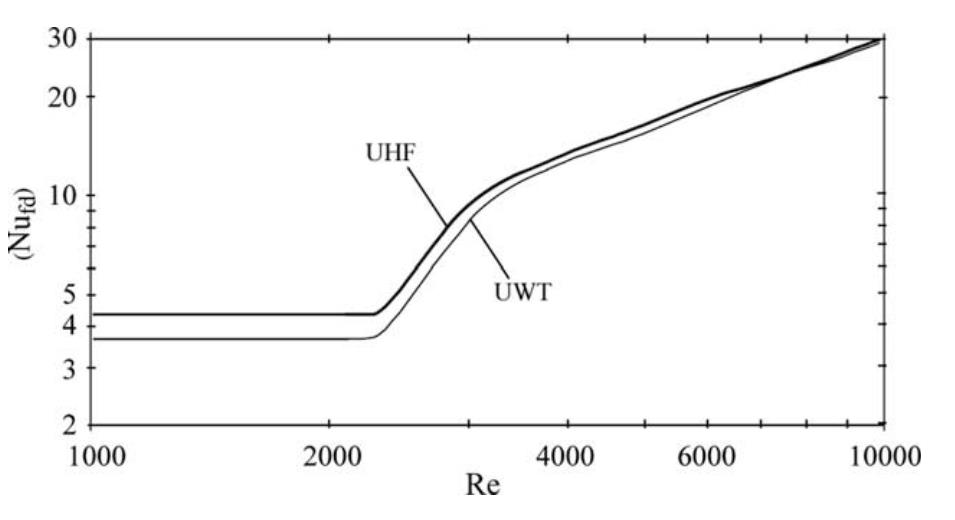
\includegraphics[scale=0.3]{figures/nusselt}
  \caption{Závislost Nusseltova čísla na Reynoldsově čísle \cite{Abraham2009}}
  \label{fig:NuReynolds}
\end{figure}

Hodnotu Nusseltova čísla je možné určit na základě vztahů jak pro rovnoměrné
rozložení teploty na stěně (označováno jako UWT), tak pro rovnoměrné rozložení
tepelného toku (označované jako UHF). Dle \cite{Abraham2009} je pro všechny
režimy proudění vhodné používat následující model Nusseltova čísla:
\begin{equation}
\label{eq:NuModel}
  Nu =
  \begin{dcases}
    c_0 & Re\leq 2300 \\
    \sum_{i=1}^{5} c_i\left(\frac{Re}{10^3}\right)^{5-i} & 2300 < Re\le 3100 \\
    \frac{\frac{f}{8}(Re-1000)Pr}
    {1+12.7{\frac{f}{8}}^{(1/2)}(Pr^{(2/3)}-1)} & 3100 < Re
  \end{dcases}
\end{equation}
kde \(Pr\) je Prandtlovo číslo (vlastnost tekutiny) a \(f\) je Darcy-Weisbachův
koeficient tření, který je popsán v podkapitole \ref{sec:PressureLoss} (skrze
něj se projevuje vliv drsnosti). Jednotlivé hodnoty parametrů tohoto modelu
jsou:
\begin{table}[H]
  \label{tab:NuModel}
  \caption{Parametry modelu Nusseltova čísla}
  \vskip6pt
  \centering
  \begin{tabular}{ccc}
    \toprule
    Parametr & UWT & UHF \\ [0.5ex]
    \hline
    \(c_0\) & 3,66 & 4,36 \\
    \(c_1\) & 3,52 & 2,2407 \\
    \(c_2\) & 45,148 & 29,499 \\
    \(c_3\) & 212,13 & 142,32 \\
    \(c_4\) & 427,45 & 292,51 \\
    \(c_5\) & 316,08 & 219,88 \\
    \bottomrule \\[0.1mm]
  \end{tabular}
\end{table}
V případě, že je teplota vnitřního povrchu potrubí známa je možné na základě
rovnic \ref{eq:ConvHeatTransfer} až \ref{eq:NuModel} určit intenzitu výměny
tepla v konkrétním okamžiku. Teplota tohoto povrchu je však ovlivněna tepelnou
hmotou jež obklopuje fluidní region (např. ocelová trubka, izolace, zemina
pod.) a tudíž je nutno korektně matematicky zachytit tepelnou dynamiku v tomto
okolí (viz~kapitola \ref{sec:SurroundingMass}).

\section{Fluidní region - tlakové ztráty/akcelerace tekutiny}
\label{sec:PressureLoss}
Tlakové vlny se v potrubí šíří výrazně rychleji (rychlostí zvuku) než vlny
teplotní (přibližně rychlost proudění tekutiny), což znamená, že lokální
události probíhají v daleko kratším časovém měřítku. Z tohoto důvodu je potřeba
v simulacích s tlakovými pulsacemi využívat krátký časový krok. Predikce
tlakových vln je užitečná pouze z hlediska ochrany proti poškozením, která
jsou způsobena tlakovými rázy a na vývoj distribuce tepla nemá výraznější vliv.
Při zanedbání rychlých tlakových pulsací lze akceleraci tekutiny podél potrubí
modelovat pomocí následující PDR:

\begin{equation}
  \label{eq:momentum}
  \frac{du}{dt} = -\frac{dp}{dx} - \frac{1}{2}\frac{f}{D}u|u|
\end{equation}
kde \(p\) je tlak a \(D\) je vnitřní průměr potrubí. Hodnotu třecího
koeficientu \(f\) lze určit z explicitní Churchilovy rovnice \ref{eq:Churchill}
\cite{Churchill1977}, která je relativně přesná pro všechny režimy proudění.

\begin{equation}
  \label{eq:Churchill}
  \begin{gathered}
    f=8\left(\left(\frac{8}{Re}\right)^{12}+(A+B)^{-1.5}\right)^\frac{1}{12} \\
    A=\left(2.457\ln\left(\left(\frac{7}{Re}\right)^{0.9}
      +0.27\frac{\epsilon}{D}\right)^{-1}\right)^{16} \\
    B=\left(\frac{37530}{Re}\right)^{16}
  \end{gathered}
\end{equation}
kde \(\epsilon\) je drsnost vnitřního povrchu potrubí a \(D\) je vnitřní průměr
potrubí.

\section{Okolní hmota – kovová stěna, izolace, zemina}
\label{sec:SurroundingMass}
Pro popis vedení tepla v okolí fluidního regionu potrubí je vhodné využít
obecnou PDR vedení tepla \ref{eq:HeatEq} v obecném \(\mathcal{R}^n\) prostoru.
\begin{equation}
  \label{eq:HeatEq}
  \frac{dT}{dt}\rho{c_p}=\nabla(\lambda\nabla{T})+S
\end{equation}
kde \(\rho\) je hustota, \(c_p\) je měrná tepelná kapacita, \(\lambda\) je
tepelná vodivost, \(T\) je teplota a \(S\) je zdroj tepla. Tato rovnice platí
pro všechny souřadnicové systémy, jelikož pro každý souřadnicový systém
existuje konkrétní varianta operátoru \(\nabla\). Dále je třeba uvažovat
okrajové podmínky zajišťující reflektující interakci \todo{se zbytkem světa}.
\begin{itemize}
  \item
    \textbf{Okrajové podmínky pro nadzemní potrubí} musí reflektovat interakci
    vnějšího povrchu rozvodů s okolním vzduchem. Dle aktuálních povětrnostních
    podmínek se tedy jedná o přenos tepla přirozenou či nucenou
    konvekcí tepla. Jde tedy o okrajovou podmínku třetího řádu (Robinovu). 
  \item
    \textbf{Okrajové podmínky pro podzemní potrubí} musí reflektovat jak
    interakci s prostředím, které se nachází nad povrchem země (to může být
    samotný vzduch nebo městská infrastruktura, budovy apod.) tak s dostatečně
    vzdálenou zeminou jak v horizontálním tak vertikálním směru. Jedná se tedy
    o tři různé okrajové podmínky. Dle \todo{cite source} je nevhodnější použít
    okrajovou podmínku prvého řádu (Dirichletovu) pro spodní okraj uvažované
    domény a podmínky druhého řádu (Neumannovu) pro oba její vertikální okraje.
    Okrajová podmínka na horním okraji je pak řádu třetího podobně jako u
    nadzemního potrubí nebo řádu čtvrtého v případě přítomnosti městské
    infrastruktury (z hlediska numerického řešení jsou si podmínky třetího a
    čtvrtého řádu velmi podobné).
\end{itemize}

\begin{figure}[!tbph]
  \centering
  \begin{minipage}{.35\textwidth}
    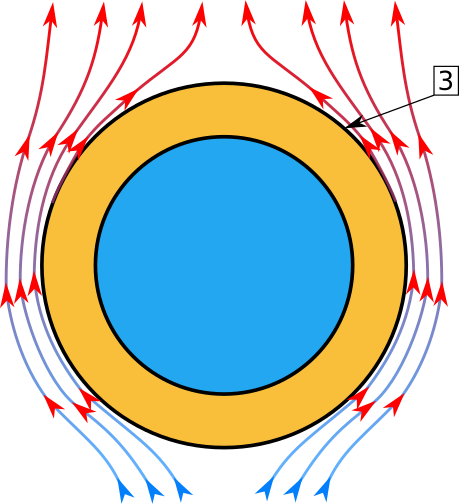
\includegraphics[width=\textwidth]{figures/above_ground_pipe}
    \caption{Nadzemní potrubí}
    \label{fig:above_ground_pipe}
  \end{minipage}
  \begin{minipage}{.55\textwidth}
    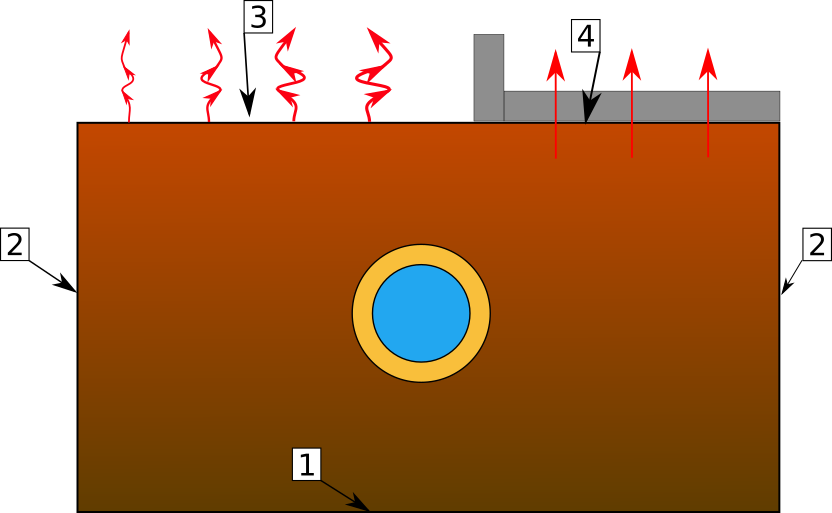
\includegraphics[width=\textwidth]{figures/burried_pipe}
    \caption{Podzemní potrubí}
    \label{fig:burried_pipe}
    \end{minipage}
\end{figure}

\section{Vlastnosti média a materiálu}
Vlastnosti tekutiny a materiálů jež vystupují v rovnicích \ref{eq:AdvDiff} až
\ref{eq:HeatEq} jsou ve skutečnosti závislé na teplotě a na tlaku (nebo
obecněji na stavových veličinách). Existují implementace programů mezinárodní
asociace pro vlastnosti vody a páry (IAPWS) \cite{IAPWS2007}, které popisují
vlastnosti vody a páry velmi přesně. Při uvažování nestlačitelnosti vody jsou
vlastnosti jako hustota, či viskozita stále výrazně proměnlivé s teplotou. Pro
tuhé skupenství je zpravidla dostačující popis polynomiální funkcí nebo i
konstantou. Při popisu zeminy se může výrazně projevit vliv její vlhkosti, což
znamená, že její vlastnosti jsou proměnlivé v čase.

\begin{figure}[h] \centering \capstart
  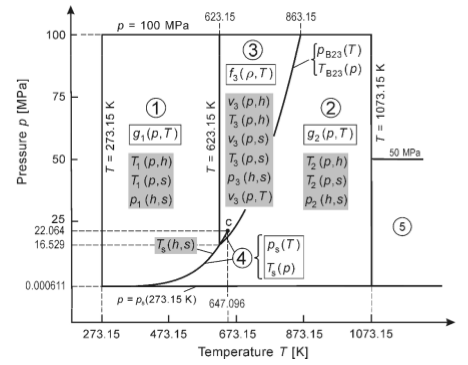
\includegraphics[scale=0.7]{figures/IF97}
  \caption{Regiony implementace vlastností vody a páry IF97 \cite{IAPWS2007}}
  \label{fig:IF97}
\end{figure}

\section{Numerické řešení a rychlost simulací}
\label{sec:NumSpeed}
V rovnicích \ref{eq:AdvDiff}, \ref{eq:momentum} a \ref{eq:HeatEq} vystupují
diferenciální operátory, jež jsou fundamentální příčinou numerické náročnosti
simulací. I přesto, že je fyzika popsaná v sekcích \ref{sec:HeatDynamics},
\ref{sec:PressureLoss} a \ref{sec:SurroundingMass} výrazně zjednodušena, je
tyto PDR nutné diskretizovat v prostoru a čase (tzv. linearizovat problém). Lze
využít metody jež jsou určeny a optimalizovány přímo pro daný kontext.
Například pro rovnici \ref{eq:AdvDiff} lze využít integrační metody vyvinuté v
NASA, které využívají aproximace derivací vyšších řádů, nežli je v samotné PDR.
Takové řešení lze nalézt např. v \cite{leonard1988}, kde jedním z
nejefektivnějších schémat je ULTIMATE QUICKEST.

Avšak mnohem častější postup při řešení PDR je její převedení na systém
ordinárních diferenciálních rovnic (ODR), jež je dále integrován (simulován) v
čase pomocí separátních algoritmů. PDR jsou v prostoru nejčastěji linearizovány
pomocí metody konečných diferencí (MKD), metody konečných objemů (MKO) či
metod konečných prvků (MKP). Pro sestavení matic a následnou integraci v čase
existuje celá řada komerčních nástrojů s přednastavenými řešiči pro jednotlivé
systémy PDR. Z Open-Source projektů zabývajícími se automatizovaným řešení PDR
je vhodné zmínit FeniCS \cite{AlnaesBlechta2015a}, kterým je možné řešit PDR
pomocí MKP (umožňuje i tzv. nespojitou Galerkinovu metodu, která je vhodná i
pro fluidní dynamiku). Tato knihovna umožňuje velmi detailně kontrolovat jakým
způsobem jsou sestavovány matice, jaké konečné elementy jsou využívány, jakým
způsobem bude během výpočtů manipulováno s objekty lineární algebry a mnoho
dalšího.

Výsledkem procesu linearizace je systém lineárních rovnic z pravidla
reprezentovaný v maticové formě. Velikost a hustota (podíl nenulových hodnot)
těchto matic pak přímo ovlivňují rychlost simulace, neboť přímo korespondují s
počtem CPU cyklů, které musí procesor (či procesory) využít na aritmetické
operace během jednoho časového kroku. V případě, že je výsledný systém
nelineární (např. jsou-li tepelné vlastnosti závislé na teplotě) je tento vliv
ještě umocněn. Pro integraci v čase existují explicitní či implicitní algoritmy
s konstantním nebo adaptivním časovým krokem. Jedny z nejefektivnějších
algoritmů jsou součástí knihovny SUNDIALS \cite{sundials}, která je
implementována v jazyce C.

\section{Vliv programovacích jazyků na modelování procesů}
\label{sec:proglang}
Programovací jazyky využité v jednotlivých modulech simulací mohou výrazně
ovlivnit výpočtovou rychlost.
\begin{itemize}
  \item
    \textbf{Kompilované jazyky} jako jsou C, C++ či Fortran jsou zpravidla
    jedny z nejrychlejších, avšak za cenu náročnějšího často velmi
    nízkoúrovňového programovaní. Tato náročnost je způsobena faktem, že tyto
    jazyky (zejména jazyk C), jsou ''mnohem~blíže'' hardwaru. Programátor musí
    například staticky určit všechny typy proměnných a také zabezpečit, že
    nedojde k nesprávnému přístupu do paměti počítače.
  \item
    \textbf{Interpretované jazyky} jako Python či Matlab jsou z hlediska
    programovaní mnohem jednodušší protože poskytují výrazně vyšší úroveň
    abstrakce a existuje k nim velké množství modulů a knihoven. Úkol spojený s
    hlídáním datových typů proměnných a správnosti přístupů do paměti počítače
    zajišťuje tzv. interpretr (interpretr pro Python je zkompilovaný C program
    zvaný CPython) a programátor má výrazně ''jednodušší život'', protože se
    může soustředit pouze na vysokoúrovňový koncept výpočtů. Programy (nebo
    přesněji skripty) napsané v těchto jazycích jsou však kvůli práci
    interpetru až o dva řády pomalejší o proti svým kompilovaným protějškům.
  \item
    Nový \textbf{Just-in-time kompilovaný jazyk} Julia \cite{julia2017}
    dosahuje rychlosti srovnatelné s jazykem C, ale zároveň poskytuje velmi
    vysokou úroveň abstrakce. Jednotlivé varianty funkcí (určeno dle typu
    argumentů, které vstupují do funkce) jsou průběžně kompilovány. Julia
    udržuje v paměti, které verze jsou již zkompilovány a které nikoliv.
    To znamená, že každé další použití již zkompilované varianty se bude chovat
    velmi podobně jako běžný kompilovaný objekt a čas potřebný na interpretaci
    v tomto okamžiku již není relevantní. Nevýhoda jazyku Julia oproti výše
    zmíněným interpretovaným jazykům spočívá v jeho novosti, což znamená, že
    mnoho vysokoúrovňových knihoven neexistuje nebo nejsou ve stavu ve kterém
    se na ně lze spoléhat.
\end{itemize}
Všechny výše zmíněné jazyky jsou \textbf{imperativní} (programy jsou definované
sekvence výpočtových kroků), avšak existují i \textbf{deklarativní} programovací jazyky
ve kterých programátor definuje logické a matematické výroky mezi objekty a
konkrétní výpočtové posloupnosti jsou vytvářeny počítačem. To znamená, že
programy mohou být z principu spouštěny libovolným směrem. Jeden z takových jazyků je například
modelica, který byl vyvinut pro matematické modelování systémů složených z
interagujících komponent. OpenModelica \todo{cite OM} je open-source verze
kompilátoru, který překládá modely ze syntaxe modelica do imperativních jazyků
(např. jazyka C) a automaticky linkuje vůči knihovnám jako jsou právě SUNDIALS
z kapitoly \ref{sec:NumSpeed}. Standardní knihovna modelica (MSL) také obsahuje
implementaci vlastností vody dle standardu IF97 (standart IAPWS). Simulace jsou
pak relativně rychlé a také velmi modulární.

\section{Počítačové učení a jeho vztah k modelování procesů}
\label{sec:ML}
\begin{figure}[h] \centering \capstart
  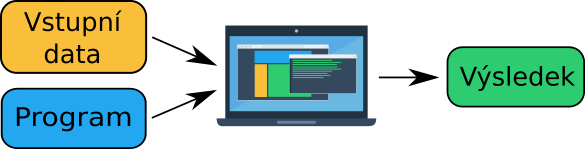
\includegraphics[scale=0.6]{figures/traditional_prog_cz}
  \caption{Tradiční programování}
  \label{fig:traditional_prog}
\end{figure}

\begin{figure}[h] \centering \capstart
  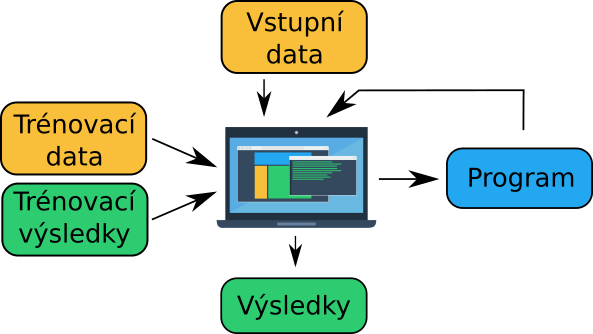
\includegraphics[scale=0.6]{figures/machine_learning_cz}
  \caption{Počítačové učení}
  \label{fig:machine_learning}
\end{figure}
Počítačové učení (anglicky machine learning) je metoda tvorby programů. Jedná
se o postup kdy je program (nebo jeho část) vytvořen počítačem. Tato oblast se
dále dělí na následující oblasti:
\begin{itemize}
  \item
    \textbf{Supervised learning} je metoda učení, která využívá člověkem
    přiřazené výsledky ke vstupním trénovacím datům. Typickým příkladem je
    klasifikace na základě znaků v datech. Trénovací data obsahují člověkem
    vytvořené anotace s požadovanými výsledky.
  \item
    \textbf{Unsupervised learning} je metoda kdy nejsou data nijak označena,
    ale algoritmus odhaluje klíčové znaky samostatně bez pomoci člověka.
    Typickým příkladem je autoenkódování.
  \item
    \textbf{Reinforcement learning} je metoda kdy prostředí ve kterém program
    operuje poskytuje informace o dopadu zásahů tohoto programu na dané
    prostředí. Typickým příkladem může být řídící člen (agent) v simulaci.
\end{itemize}
Programy v machine learning jsou v podstatě
parametrizované matematické struktury a optimalizací jejich parametrů je možné
měnit/zlepšovat chování programu. Tyto programy dále obsahují tzv.
hyperparametry, kterými se řídí struktura a komplexnost programů.

Poměrně velký úspěch v této oblasti zaznamenaly tzv. neuronové sítě (NN). Jsou
totiž velmi univerzálními aproximátory matematických funkcí, což je jejich
velkou výhodou. Jejich nevýhodou je naopak poměrně náročný proces učení a také
fakt, že vyžadují poměrně velké množství dat.

Nedávno (2019) se objevily vědecké práce, které navrhují a demonstrují využití
NN (nebo obecně parametrizovaných programů) pro matematické modelování ODR
systémů (a tudíž i PDR) \cite{diffEqFlux2019, chen2018neural}. Ukázkové modely
byly v těchto dvou implementacích prováděny akcelerovanou metodou gradient
descend, přičemž gradient byl určen algoritmickou zpětnou propagací skrze ODR
solver (což je největším přínosem těchto prací). Gradient descend je obecně
považován za nejvíce pokročilou metodu učení modelů, avšak je poměrně náročný
na implementaci.

Existují i algoritmy jež nevyžadují derivace a jsou vhodné pro modely, u
kterých nelze derivace určit. Tyto algoritmy umožňují optimalizaci až na úrovni
black box.

Machine learning a mechanistické modelování na základě PDR lze tedy kombinovat.
Tímto je možné modelovat procesy na základě experimentálních dat, zjednodušovat
komplexnost programů na základě extrahovaných veličin z více komplexních
simulací nebo optimalizovat (ladit) zmámé mechanistické struktury pomocí
experimentálních dat.


\chapter{Analýza, interpretace a zhodnocení poznatků získaných na základě
kritické rešerše}
\textbf{Příklad}:
